\documentclass{amsart}
\usepackage{../../../lucas}
\usepackage{amsmath, amssymb}
\usepackage{graphicx}
\graphicspath{ {./images} }

\title{Problem Set 5}
\author{Lucas\ Chen}
\date{\today}
\begin{document}

\maketitle



\subsection*{Problem 5} Suppose that \( f_n : [a, b] \to \mathbb{R} \) and \( f_n \rightrightarrows f \) as \( n \to \infty \). Which of the following discontinuity properties (see Exercise 3.36) of the functions \( f_n \) carries over to the limit function? (Prove or give a counterexample.)

(a) No discontinuities.

\medskip \noindent $f_n$ are continuous and therefore $f$ is continuous by textbook Theorem 1. Property carries over.

\bigskip

(b) At most ten discontinuities.

\medskip \noindent Property carries over. Assume $>10$ discontinuities in $f(x)$. Then there are at least $a>10$ intervals with
discontinuities in $f(x)$. Take the sequence restricted to the $i^{\text{th}}$ interval, $(f_{ni})$. If there are infinitely many $n$
where $f_{ni}$ is continuous, take those $n$ as a subsequence, which must converge to $f_i$ the same limit as the overall sequence,
which is discontinuous: the subsequence remains uniformly convergent and yields a contradiction.

\medskip \noindent Thus there can only be finitely many elements of the sequence continuous on each interval. Select an arbitrary
11 intervals. Then take the maximum number of $n$ where $f_{ni}$ are continuous across the eleven intervals and call it $b$: the total number of 
continuous functions in the set is at maximum $11b$, and there are at maximum $11b$ values of $n$ where
only $10$ intervals are discontinuous. Thus there exists some $n$ where $11$ intervals are discontinuous and the property must 
carry by contrapositive.

\bigskip

(c) At least ten discontinuities.

\medskip \noindent Property does not carry over: consider the sequence $(f_n(x))$ on $[-10, 10]$ with \[f_n(x)=\begin{cases}
    1/n & \text{if } \lceil n\rceil \text{ is even,}\\
    -1/n & \text{ otherwise.}
\end{cases}\]
These functions have infinitely many discontinuities but converge uniformly to $f(x)=0$, which is continuous.

\bigskip

(d) Finitely many discontinuities.

Does not carry over because you can end up with infinitely many. (take one more discontinuity each time and end up
with countably infinite number)

For example, take \[f_n(x) = \lfloor nx\rfloor/n\] on $[-5, 5]$ which has $10n+1$ discontinuities for each $n$
but uniformly converges to $f(x)=x$. 

\bigskip

(e) Countably many discontinuities, all of jump type.

\medskip \noindent Take $c$ in $[a,b]$. We prove $\lim_{x\to c^+}f(x)$ and $\lim_{x\to c^-}f(x)$ exist and
are equal to $\lim_{n\to\infty} r_n$ and $\lim_{n\to\infty} l_n$ for $r_n=\lim_{x\to c^+}f_n(x)$
and $l_n=\lim_{x\to c^-}f_n(x)$ which exist since $f_n$ has only jump discontinuities. 

\medskip \noindent First we prove that $r_n$ and $l_n$ are Cauchy. We prove this for $l_n$ and the proof for $r_n$ is analogous.
Take $\epsilon>0$. For each $n$ take $\delta_n$ where if $x'\in (c-\delta_n, c)$ then $d(f_n(x'), l_n)<\epsilon/3$. Now since
$f_n$ is uniformly continuous (and Cauchy) we take $N$ such that $d(f_p, f_q)<\epsilon/3$ for $p, q>N$. Take 
$x'\in (\max(c-\delta_p, c-\delta_q), c)$. Then for $p, q>N$ we have \[d(l_p, l_q)\leq d(l_p, f_p(x'))+d(f_p(x'), f_q(x'))+d(f_q(x'), l_q)<\epsilon. \]
Thus $l_n$ is Cauchy and converges since it is in $\mathbb{R}$; call the limit $l$. 

\medskip \noindent We prove $\lim_{x\to c^-}f(x)=l$.  
Take $M_1$ so that $d(f_{p_1}, f)<\epsilon/3$ for $p_1>M_1$ and $M_2$ so that $d(l_{p_2}, l)<\epsilon/3$
for $p_2, q_2>M_2$. Take $n>M_1,M_2$. Then take $\delta$ so that for $x'\in (c-\delta, c)$, $d(l_n, f_n(x'))<\epsilon/3$. 
Then for $x'\in (c-\delta, c)$ we have \[d(f(x'), l)\leq d(f(x'), f_n(x'))+d(f_n(x'), l_n) + d(l_n, l) < \epsilon\] and $l$ is 
the left limit of $f$ at $c$. The right argument is analogous, so $f$ has left and right limits at every point and therefore no
oscillating discontinuities. By problem 36 on pset 4 we know there can be at most a countable number of jump discontinuities so
the property must carry.

\bigskip

(f) No jump discontinuities.

\medskip \noindent Property does not carry over. Just take two oscillating discontinuities that end at different points and squeeze them
into jump discontinuities.

\bigskip

(g) No oscillating discontinuities.

\medskip \noindent If (e) carries than (g) carries by problem 36 of pset 4, since there can only be countably many jump discontinuities in each
$f_n$.

\newpage

\subsection*{Problem 8} Is the sequence of functions \( f_n : \mathbb{R} \to \mathbb{R} \) defined by
    \[
    f_n(x) = \cos(n + x) + \log \left( 1 + \frac{1}{\sqrt{n + 2}} \sin^2(n^n x) \right)
    \]
equicontinuous? Prove or disprove.

\medskip \noindent \textbf{Lemma 1}: If $g_n$ is equicontinuous, $f_n$ is uniformly continuous for all $n\in \mathbb{N}$, and $\lim_{n\to \infty}d(f_n, g_n) = 0$
then $f_n$ is equicontinuous.

\medskip \noindent \textbf{Proof of Lemma 1}: Take $\epsilon>0$. Then there exists $N\in \mathbb{N}$ where $n>N\implies d(f_n, g_n)<\epsilon/3$. By
equicontinuity of $g_n$ we take $\delta_g$ where $|s-t|<\delta_g\implies d(g_n(s), g_n(t))<\epsilon/3$. Then for $|s-t|<\delta_g$
and $n>N$, we have \[d(f_n(s), f_n(t))\leq d(f_n(s), g_n(s))+d(g_n(s), g_n(t))+d(g_n(t), f_n(t))<3\epsilon/3=\epsilon\] by triangle inequality.

\medskip \noindent For $m\leq N$ we take $\delta_m$ where
$|s-t|<\delta_m\implies d(f_m(s), f_m(t))<\epsilon$. Then take an overall $\delta = \min(\delta_g, \min_{m<N}(\delta_m))$ which
ensures that $d(s,t)<\delta\leq \delta_g, \delta_m\implies d(f_a(s), f_a(t))<\epsilon$ for each $a\in\mathbb{N}$. Thus $f_n$ is equicontinuous.

\medskip \noindent \textbf{Proof of 8}: We prove $\cos(n+x)$ is equicontinuous, $f_n$ is uniformly continuous, and 
$\lim_{n\to\infty}\log(1+\frac{\sin^2(n^nx)}{\sqrt{n+2}})=0$.

\medskip \noindent For $\cos(n+x)$ take $\delta=\epsilon$ for $\epsilon>0$. Then if $d(s, t)<\delta$ and 
$d(\cos(n+s),\cos(n+t))\geq\epsilon$ we have \[\frac{|\cos(n+s)-\cos(n+t)}{|(n+s)-(n+t)|}>1\] which is impossible
by mean value theorem, since the derivative of $\cos$ is bounded in $[-1, 1]$. Thus $\cos(n+x)$ is equicontinuous.

\medskip \noindent For the third statement we prove \[0\leq\log \left( 1+\frac{\sin^2(n^nx)}{\sqrt{n+2}} \right)\leq \log \left( 1+\frac{1}{\sqrt{n+2}} \right) \leq \frac{1}{\sqrt{n+2}}\]
which by squeeze theorem will yield $\lim_{n\to\infty}\log(1+\frac{\sin^2(n^nx)}{\sqrt{n+2}})=0$. We have $\sin^2(n^nx)\in [0,1]$. $\log(1+a)\leq a$ for
nonnegative $a$: we have $1+a\leq e^a=\sum_{m=0}^{\infty}\frac{a^m}{m!}$ where $\sum_{m=2}^{\infty}\frac{a^m}{m!}$ is positive,
and since $e^x$ is increasing ($(e^x)'$ is always positive) this implies the inequality above.

\medskip \noindent To prove $f_n$ is uniformly continuous we note that $\forall n$ $f_n(x)= f_n(x+2\pi m)$ for $m\in \mathbb{Z}$. Then consider $f_n$ restricted to the 
domain $[-2\pi, 2\pi]$. This function is continuous since it is the composition of continuous functions, and since it is
on a compact interval it must be uniformly continuous. We extrapolate the uniform continuity condition to $\mathbb{R}$. Take $\epsilon>0$ and 
take the corresponding $\delta$ from $f_{n[-2\pi, 2\pi]}$. For $|s-t|<\min(2\pi, \delta)$ we consider $s-2\pi(\lfloor \frac{s}{2\pi}\rfloor)$. WLOG assume $s>t$. Then we have two cases:

\medskip \noindent 1) $\lfloor \frac{s}{2\pi}\rfloor = \lfloor \frac{t}{2\pi}\rfloor$, in which case $s-2\pi(\lfloor \frac{s}{2\pi}\rfloor)$ and $t-2\pi(\lfloor \frac{t}{2\pi}\rfloor)$ are in $[0, 2\pi]$ and 
$d(f_n(s-2\pi(\lfloor \frac{s}{2\pi}\rfloor)), f_n(t-2\pi(\lfloor \frac{t}{2\pi}\rfloor)))<\epsilon$ implies $d(f_n(s), f_n(t))<\epsilon$ if $|s-t|=|s-2\pi(\lfloor \frac{s}{2\pi}\rfloor)-(t-2\pi(\lfloor \frac{t}{2\pi}\rfloor))|<\delta$. 

\medskip \noindent 2) $\lfloor \frac{s}{2\pi}\rfloor = 1+\lfloor \frac{t}{2\pi}\rfloor$. No other cases are possible because $s-t<2\pi$. In this case $s-2\pi(\lfloor \frac{s}{2\pi}\rfloor)$ is in $[0, 2\pi]$
and $t-2\pi(\lfloor \frac{s}{2\pi}\rfloor)=t-2\pi(\lfloor \frac{t}{2\pi}\rfloor+1)$ is in $[-2\pi, 0]$. Once again for $|s-2\pi(\lfloor \frac{s}{2\pi}\rfloor)-(t-2\pi(\lfloor \frac{s}{2\pi}\rfloor))|<\delta$ the uniform
continuity condition of the restricted function provides $d(f_n(s), f_n(t))<\epsilon$. Thus $f_n$ is uniformly continuous for each $n$ and by Lemma 1 we 
have $f_n$ equicontinuous.

\newpage

\subsection*{Problem 9} If \( f : \mathbb{R} \to \mathbb{R} \) is continuous and the sequence \( f_n(x) = f(nx) \) is equicontinuous, what can be said about \( f \)?

\medskip \noindent $f$ is constant. If $f$ is not constant then $\exists$ $f(x_1)\neq f(x_2)$. Take $\epsilon$ less than $|f(x_1)-f(x_2)|$. For any $\delta$
proposed for the equicontinuity condition we take $n> \frac{|x_1-x_2|}{\delta}$. Then $f_n(x_1/n)=f(x_1), f_n(x_2/n)=f(x_2)$. Then $\frac{|x_1-x_2|}{n}<\delta$ but 
$f(x_1)-f(x_2)>\epsilon$ which is a contradiction.



\newpage

\subsection*{Problem 15} A continuous, strictly increasing function \( \mu : (0, \infty) \to (0, \infty) \) is a \textit{modulus of continuity} if \( \mu(s) \to 0 \) as \( s \to 0 \). A function \( f : [a, b] \to \mathbb{R} \) has modulus of continuity \( \mu \) if \( |f(s) - f(t)| \leq \mu(|s - t|) \) for all \( s, t \in [a, b] \).

(a) Prove that a function is uniformly continuous if and only if it has a modulus of continuity.

\medskip \noindent Take $\epsilon>0$. We have $\delta$ such that $s<\delta$ implies $\mu(s)<\epsilon$. Take
$|s-t|<\delta$. Then $\mu(|s-t|)<\epsilon$ implies $|f(s)-f(t)|<\epsilon$ and the uniform continuity condition is satisfied.

\medskip \noindent Take uniform continuity. Then define \[\mu(s) = s+\sup\{d(f(x_1), f(x_2)) : d(x_1, x_2)<s\}.\] $\mu$ is well-defined
because $d(f(x_1), f(x_2))$ is bounded above, since the range is the continuous image of a compact set. Since 
$\{x_1, x_2: d(x_1,x_2)<s\}\subset \{x_1, x_2: d(x_1, x_2)<t\}$ for $s<t$, $\mu(s)<\mu(t)$ for $s<t$; since distances
are always positive the function's domain and range are both $(0, \infty)$, and since continuous functions
map Cauchy (convergent) sequences to Cauchy sequences, $\lim_{s\to 0} \mu(s) = 0$ ($f(s)$ and $f(t)$ must get arbitrarily
close as $s$ and $t$ do).

\medskip \noindent We now prove continuity of $\mu$ (or rather $\mu_f(s)=\mu-s$ which implies continuity of $\mu$). Consider left-continuity first. Take $\epsilon>0$. 
We prove that $\exists \delta$ where $t\in (s-\delta, s)$ implies $\mu_f(t)>\mu_f(s)-\epsilon$ (since $\mu_f$ is increasing). Increasing
$\mu_f$ implies that if there exists any such $t$ then all elements of $[t, s)$ satisfy the condition. Since the distance function is a continuous
function of $f([a,b])\times f([a,b])$ it achieves a supremum and we can select $x_1, x_2$ with $d(x_1, x_2)=s$ and $d(f(x_1), f(x_2))\geq\mu_f(s)$ 
(since the supremum for $d(x_1, x_2)=s$ is the supremum for $d(x_1, x_2)\leq s$ and exceeds the supremum of $d(x_1, x_2)<s$ via nested sets). Fix $x_2$. 
$\exists \delta_{\mu}$ such that for $d(x_1, a)<\delta_{\mu}$, $d(f(x_1), f(a))<\epsilon$. Then take $a\in (x_1, x_2)$. We have
\[d(f(x_1), f(x_2))\leq d(f(x_1), f(a))+d(f(a), f(x_2))<d(f(a), f(x_2))+\epsilon\]
\[\implies \mu_f(s)-\epsilon<d(f(a), f(x_2))\leq \mu(d(a, x_2))\] and since $a\in (x_1, x_2)$ we have $t=d(a, x_2)<s$ and left-continuity.

\medskip \noindent Now consider right-continuity. We similarly look for a $t>s$ such that $\mu_f(t)<\mu_f(s)+\epsilon$. Take $\delta_{\mu}$ where 
$d(x_1, x_2)<\delta_{\mu}\implies d(f(x_1), f(x_2))<\epsilon$ for arbitrary $x_1, x_2$. Then for $\mu_f(s+\delta_{\mu})$ any $y_1 \leq y_2$ with
$d(y_1, y_2)<s+\delta_{\mu}$ we pick $y_3=\max(y_1, y_2-\delta_{\mu})$, where $d(y_1, y_3)<s$. Then 
\[d(f(y_1), f(y_2))\leq d(f(y_1), f(y_3))+d(f(y_3), f(y_2))<d(f(y_1), f(y_3))+\epsilon\leq\mu_f(s)+\epsilon.\]
Since $\mu_f(t)=\mu_f(s+\delta_{\mu})=\sup\{d(f(y_1), f(y_2))\}$, $\exists y_1, y_2$ where $\mu_f(t)-\epsilon_2<d(f(y_1), f(y_2))$ for each $\epsilon_2$.
Then pick some $c\in (d(f(y_1), f(y_2)), \mu_f(s)+\epsilon))$. $\mu_f(t)<c+\epsilon_2$ for all $\epsilon_2$ implies
$\mu_f(t)\leq c$ by $\epsilon$-principle, which in turn implies $\mu_f(t)<\mu_f(s)+\epsilon$ and right-continuity. Thus $\mu_f$ and 
therefore $\mu$ are continuous.

\bigskip

(b) Prove that a family of functions is equicontinuous if and only if its members have a common modulus of continuity.
    
\medskip \noindent Take equicontinuous family $\mathcal{E}$. For the forward direction once again take $\delta$ for each $\epsilon$ where $s<\delta$ implies $\mu(s)<\epsilon$.
Then the proof follows exactly the same: $|s-t|<\delta$ implies $|f(s)-f(t)|\leq \mu(|s-t|)<\epsilon$ for each $f$ in the family since
they each have the same modulus.

\medskip \noindent Construct modulus of continuity \[\mu(s)=s+\sup\{d(f(x_1), f(x_2)): d(x_1, x_2)<s, f\in\mathcal{E}\}.\] This function is well defined:
say that for some $s$ there is no $\epsilon$ that bounds $d(f(x_1), f(x_2))$ from above with $d(x_1, x_2)<s$. Pick an arbitrary $\epsilon_1$. Then $\exists$ a
$\delta$ where $d(y_1, y_2)<\delta$ implies $d(f(y_1, y_2))<\epsilon_1$ for each $f$ and each $y_1, y_2$: for any $x_1, x_2$ where $d(x_1, x_2)<s$ we can take
the minimum $n\in \mathbb{N}$ where $x_1+nd>x_2$, with $d<\delta$. Then $d(f(x_1), f(x_2))< (\sum_{i=0}^{n-2}d(f(x_1+id), f(x_1+(i+1)d)))+d(f(x_1+(n-1)d), f(x_2))<n\epsilon_1$ for each $f$ and thus
there does exist an upper bound $\epsilon$ and therefore a supremum.

\medskip \noindent From here the proof proceeds the exact same way since we can take the $\epsilon$ for the domain of the family
to find the maximum bounded codomain, which is compact and therefore follows the extreme value theorem. Proving left-continuity follows by picking
an $f$ along with $x_1, x_2$ and following the same steps. Proving right-continuity follows the same argument 
using the uniform continuity condition over all $f\in\mathcal{E}$.


\newpage

\subsection*{Problem 17} Consider a modulus of continuity \( \mu(s) = H s^{\alpha} \) where \( 0 < \alpha \leq 1 \) and \( 0 < H < \infty \). A function with this modulus of continuity is said to be \textit{\( \alpha \)-Hölder}, with \( \alpha \)-Hölder constant \( H \). See also Exercise 3.2.
    
(a) Prove that the set \( C^{\alpha}(H) \) of all continuous functions defined on \( [a, b] \) which are \( \alpha \)-Hölder and have \( \alpha \)-Hölder constant \( \leq H \) is equicontinuous.

\medskip \noindent If an $\alpha$-H\"{o}lder function has $\alpha$-H\"{o}lder constant $\leq H$ then it is also $\alpha$-H\"{o}lder with
$\alpha$-H\"{o}lder constant $H$, since if $\mu_H>\mu$ and $\mu$ is a modulus of continuity then $\mu_H$ also satisfies the conditions.
For a given $\epsilon$ we have that \[d(x_1, x_2)<(\epsilon/H)^{(1/\alpha)}\implies d(f(x_1), f(x_2))<\epsilon\] for all $f$ in $C^{\alpha}(H)$
and the equicontinuity condition is met.

(b) Replace \( [a, b] \) with \( (a, b) \). Is the same thing true?

\medskip \noindent This changes nothing.

\bigskip

(c) Replace \( [a, b] \) with \( \mathbb{R} \). Is it true?

\medskip \noindent This changes nothing.

\bigskip

(d) What about \( \mathbb{Q}? \)

\medskip \noindent This changes nothing (since the distance function remains mapped onto $\mathbb{R}$, and the uniform continuity definition does not require completion).

\bigskip

(e) What about \( \mathbb{N}? \)
    
\medskip \noindent This changes nothing (since the distance function remains mapped onto $\mathbb{R}$, and the uniform continuity definition does not require completion).

\newpage

\subsection*{Problem 18} Suppose that \( (f_n) \) is an equicontinuous sequence in \( C^0 \) and \( p \in [a, b] \) is given.
    
(a) If \( (f_n(p)) \) is a bounded sequence of real numbers, prove that \( (f_n) \) is uniformly bounded.

\medskip \noindent The family is equicontinuous so it has a modulus of continuity $\mu$. Take $\mu(|a-b|)$. Take an interval bound of $(f_n(p))$ 
$(c, d)$: the family is uniformly bounded by $(c-\mu(|a-b|), d+\mu(|a-b|))$ since no point in the image of $f_n$ can ever 
be more than $\mu(|a-b|)$ away from $f_n(p)$. 
\bigskip

(b) Reformulate the Arzelà-Ascoli Theorem with the weaker boundedness hypothesis in (a).

\medskip \noindent If $(f_n)$ is an equicontinuous sequence in $C^0$ and $(f_n(p))$ is bounded for some $p\in [a,b]$,
then $(f_n)$ has a convergent subsequence. The proof follows the same countable dense set argument with diagonal subsequences
as the proof in the book.

\bigskip

(c) Can \( [a, b] \) be replaced with \( (a, b)? \), \( \mathbb{Q}? \), \( \mathbb{R}? \), \( \mathbb{N}? \)

\medskip \noindent We can replace $[a, b]$ with the open interval since the family remains uniformly bounded by the same argument, but
since we use a modulus of continuity of the domain of the family to argue uniform boundedness we cannot replace the 
closed interval with any unbounded set. For each unbounded set we take the family ${f(x)=x}$ for a counterexample. 

\bigskip

(d) What is the correct generalization?

\medskip \noindent A bounded and path-connected set (since the argument in 15b relies on the path-connectedness of the domain for the 
uniform boundedness of the family).

\newpage

\subsection*{Problem 19} If \( M \) is compact and \( A \) is dense in \( M \), prove that for each \( \delta > 0 \) there is a finite subset \( \{a_1, \ldots, a_k\} \subset A \) which is \( \delta \)-dense in \( M \) in the sense that each \( x \in M \) lies within distance \( \delta \) of at least one of the points \( a_1, \ldots, a_k \).

\medskip \noindent Take set $C = \bigcup_{a\in A} B_{\delta}(a)$, which is a covering of $M$ by the density of $A$. Since $M$ is compact 
$C$ has a finite subcover and each point in $M$ is therefore within $\delta$ of a center of one of the components of the finite subcover.

\newpage

\subsection*{Problem 21} Suppose that \( \mathcal{E} \subset C^0 \) is equicontinuous and bounded.

(a) Prove that \( \sup \{ f(x) : f \in \mathcal{E} \} \) is a continuous function of \( x \).

\medskip \noindent Take $g(x) = \sup\{f(x): f\in \mathcal{E}\}$, and $\epsilon>0$. Since $g(x)$ is
a supremum, for some $x$ and $f_a\in\mathcal{E}$ we have $f_a(x)>g(x)-\epsilon/2$ (otherwise $g(x)-\epsilon/2$ is an upper bound).
Take $\delta$ such that $d(x, x_1)<\delta\implies d(f(x), f(x_1))<\epsilon/2$ for each $f\in\mathcal{E}$. Then $f\leq g$ implies $f(x_1)<g(x)+\epsilon/2$
for each $f$, so $g(x_1)\leq g(x)+\epsilon/2<g(x)+\epsilon$. We also have $g(x_1)\geq f_a(x_1)>f_a(x)-\epsilon/2>g(x)-\epsilon$. Thus $d(g(x_1), g(x))<\epsilon$
for $d(x_1, x)<\delta$.


\bigskip

(b) Show that (a) fails without equicontinuity.

\medskip \noindent Take $\mathcal{E} = (f_n)$ where \[f_n=\begin{cases}
    0 & \text{if } x<0\\
    nx & \text{if } 0\leq x < 1/n\\
    1 & \text{if } x\geq1/n
\end{cases}\]
The functions all have range $[0, 1]$ but here \[g(x) =\begin{cases}
    0 & \text{if } x\leq 0 \\
    1 & \text{otherwise.}
\end{cases}\]
since for all $x>0$ $\exists n\in\mathbb{N}$ where $1/n<x$. 

\bigskip

(c) Show that this continuous-sup property does not imply equicontinuity.

\medskip \noindent Take the function family $f_a(x) = \sin(ax)$ for $a\in\mathbb{R}$. Then for any point
$x$ we have $a=\frac{\pi}{2x}$ yields $f_a(x)=1$ and $f_a(x)\in [-1, 1]$ for each $x$. Then the supremum
of the family is $g(x)=1$. However, $\{sin(nx): n\in\mathbb{N}\}\subset$ this family and by problem 9 the 
family is not equicontinuous.

\bigskip

(d) Assume that the continuous-sup property is true for each subset \( \mathcal{F} \subset \mathcal{E} \). Is \( \mathcal{E} \) equicontinuous? Give a proof or counterexample.

\medskip Take the function family $f_n(x)=e^{-(nx)^2}$ for $n\in\mathbb{N}$. Then any subset of the family has supremum
$f_a(x)$ where $a$ is the minimum $n$ in the subset: for $a<b$ $e^{-(ax)^2}\geq e^{-(bx)^2}$. Thus it satisfies
the continuous-sup property but by problem 9 the family is not equicontinuous.

\newpage

\subsection*{Problem 24} Suppose that a sequence of continuous functions \( f_n : [a, b] \to \mathbb{R} \) converges monotonically down to a continuous function \( f \). (That is, for each \( x \in [a, b] \) we have \( f_1(x) \geq f_2(x) \geq f_3(x) \geq \dots \) and \( f_n(x) \to f(x) \) as \( n \to \infty \).)
    
(a) Prove that the convergence is uniform.

\medskip \noindent Assume convergence not uniform. Then for some $\epsilon$, for each $n$ there exists $x_n$ where $d(f_n(x_n), f(x_n))\geq \epsilon$.
Since $[a,b]$ is compact $\exists$ a convergent subsequence $x_{n_k}$ with limit $x$. For any $a>0$ and $k>a$ where
$d(f(x_{n_k}), f(x))<\epsilon/3$ and $d(f_a(x_{n_k}), f_a(x))<\epsilon/3$, which exist because $x_{n_k}$ gets
arbitrarily close to $x$ and we pick the maximum of two $k$. $k>a$ implies $f_a\geq f_k$ and $d(f_a(x_{n_k}),f(x_{n_k}))\geq d(f_k(x_{n_k}), f(x_{n_k})) \geq \epsilon$. 
Then \[d(f_a(x), f(x))+2\epsilon/3 > d(f_a(x_{n_k}), f(x_{n_k}))+d(f_a(x_{n_k}), f_a(x))+d(f(x_{n_k}), f(x))\]
\[\geq d(f_a(x_{n_k}),f(x_{n_k}))\geq \epsilon\] which yields $d(f_a(x), f(x))>\epsilon/3$ for all $a$, a contradiction.

(b) What if the sequence is increasing instead of decreasing?

\medskip \noindent Take the negative of the sequence and it is then increasing. The negative sequence
converges uniformly. Since the sup distances remain the same therefore the original sequence also converges
uniformly.

\bigskip

(c) What if you replace \( [a, b] \) with \( \mathbb{R} \)?

\medskip \noindent Take $f_n(x) = x^2/n$. This converges pointwise to $0$ but does not converge uniformly since
it is unbounded.

\bigskip

(d) What if you replace \( [a, b] \) with a compact metric space or \( \mathbb{R}^m \)?

\medskip \noindent Take $f_n(x) = x_1^2/n$ and we have the same counterexample for $\mathbb{R}^n$. A compact metric 
space does not change the result of (a) because we made only the assumption that the domain was compact.

\newpage

\subsection*{Problem 43} What is the joke in the following picture?

\bigskip

\begin{figure}[h]
    \centering
    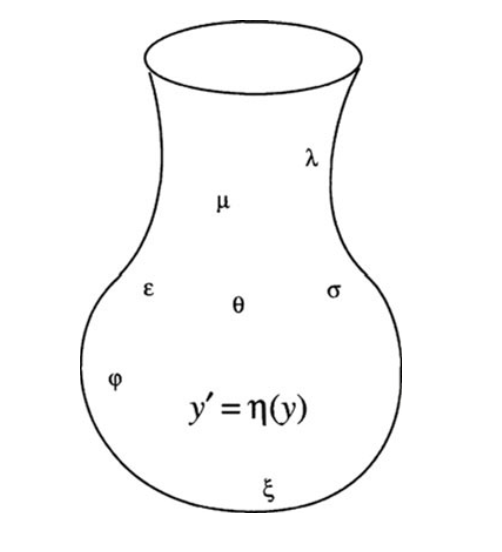
\includegraphics{joke.png}
\end{figure}

It's an ode on a Grecian urn. I tried really hard to read into the eta and the near-timelessness theme of the original
poem but came up short. I have no idea what the eta means but the only thing I can think of is a garbage
pun on eating :(


\end{document}

